\chapter{फ़ोटॉन और फ़ोनॉन}\label{ch:b3:photons-phonons}

क्वांटम सिद्धांत का जन्म इसी अध्याय के विषय में हुआ था। 1900 में
दहकते पिंडों के वर्णक्रम ने चिरसम्मत भौतिकी मानने से इनकार कर दिया ---
और उससे भी बुरा, चिरसम्मत भौतिकी छोटी तरंगदैर्घ्यों पर \emph{अनंत}
ऊर्जा की भविष्यवाणी करती थी, यानी ``पराबैंगनी विपदा'' --- और प्लांक का
हताश उपाय, अर्थात् $h\nu$ के पुलिंदों में ऊर्जा, आगे चलकर उस
सदी की मूल कुंजी निकला। अब जब यंत्र जुट चुका है ---
\cref{ch:b3:schrodinger-three-dimensions} से मोड-गणना और
\cref{ch:b3:canonical-ensemble} से दोलक की ऊष्मागतिकी --- \omterm{thm:b3:photons-phonons:planck}{प्लांक का
नियम} आधे पन्ने में निकल आता है: फ़ोटॉनों की एक गैस, प्रति गुहा-मोड एक
बोसॉनी ढंग से अधिभुक्त दोलक। वही आधा पन्ना, प्रकाश की जगह ध्वनि के
साथ, ठोसों का डिबाई सिद्धांत है और वही $T^3$ ऊष्माधारिता, जो
आइंस्टाइन का प्रतिरूप चूक गया था। और ब्रह्मांड के हर घन सेंटीमीटर को
भरे हुए है इस विषय की उत्कृष्ट कृति: 2.725 केल्विन की ब्रह्मांडीय
सूक्ष्मतरंग पृष्ठभूमि, अब तक नापी गई सबसे पूर्ण कृष्णिका --- स्वयं
युवा ब्रह्मांड का तापीय विकिरण, जो अब भी आ रहा है।

\section{प्लांक का नियम, व्युत्पन्न}

\begin{theorem}[कृष्णिका वर्णक्रम]\label{thm:b3:photons-phonons:planck}
\index{प्लांक का नियम}\index{कृष्णिका विकिरण}
ताप $T$ पर कोई गुहा विद्युत्-चुंबकीय मोड सँभालती है --- अर्थात्
अप्रगामी तरंगें, जो ठीक
\cref{prop:b3:schrodinger-three-dimensions:counting} की तरह गिनी
जाती हैं, और ध्रुवण के लिए दुगनी:
\[
g(\nu)\,\dd\nu = \frac{8\pi V}{c^3}\,\nu^2\,\dd\nu .
\]
हर मोड एक क्वांटम दोलक है, जो संतुलन पर
$\bar n = 1/(\eu^{h\nu/k_{\text{B}}T} - 1)$ फ़ोटॉन रखता है
(\cref{exo:b3:canonical-ensemble:5}; या तुल्य रूप से, $\mu =
0$ पर बोसॉन)। अतः प्रति आयतन प्रति आवृत्ति ऊर्जा है
\[
u(\nu, T) = \frac{8\pi h\nu^3}{c^3}\,
\frac{1}{\eu^{h\nu/k_{\text{B}}T} - 1} :
\]
अर्थात् \emph{\omterm{thm:b3:photons-phonons:planck}{प्लांक का नियम}} (1900)। उसके परिणाम, सब जैसे नापे गए:
शिखर $\lambda_{\max}T = \qty{2898}{\micro m.K}$ पर (वर्ष 2 के खंड
का वीन विस्थापन-नियम, अब व्युत्पन्न); किसी काली सतह से कुल अभिवाह
$\Phi = \sigma T^4$, जहाँ
\[
\sigma = \frac{2\pi^5k_{\text{B}}^4}{15h^3c^2}
 = \qty{5.67e-8}{W.m^{-2}.K^{-4}}
\]
(श्टेफ़ान--बोल्ट्ज़मान, जिसका नियतांक अब $h$, $c$,
$k_{\text{B}}$ से बना है); और फ़ोटॉन घनत्व $n_\gamma \approx
\num{2.03e7}\,(T/\unit{K})^3$ प्रति घन मीटर।
\end{theorem}

\begin{proof}[आंशिक उपपत्ति]
मोड-गणना को $h\nu\,\bar n$ से गुणा कीजिए। कुल ऊर्जा का
समाकल, $x = h\nu/k_{\text{B}}T$ और $\int_0^\infty
x^3\dd x/(\eu^x - 1) = \pi^4/15$ (मान लिया गया) के साथ, $u_{\text{कु}}
= aT^4$ देता है और, मानक अभिवाह-गुणक $c/4$ के साथ, कथित
$\sigma$। वीन का नियम \cref{exo:b3:photons-phonons:1} वाला
अधिकतमीकरण है। कम आवृत्ति पर ($h\nu \ll
k_{\text{B}}T$) हर मोड $k_{\text{B}}T$ ढोता है ---
रैले--जीन्स, जो रेडियो के लिए सही है और सभी
$\nu$ तक बढ़ा दिया जाए तो विपदाकारी: प्लांक का कटाव दरअसल
ऊर्जा-समविभाजन का लाइसेंस
(\cref{thm:b3:canonical-ensemble:equipartition}) मोड-दर-मोड रद्द
होना है।
\end{proof}

\begin{omfigure}
\begin{tikzpicture}
  \begin{axis}[omaxis, axis x line=bottom, axis y line=left,
    width=11.4cm, height=6.0cm, xmin=0, xmax=4.4, ymin=0, ymax=1.5,
    xlabel={$\nu$ ($10^{14}$ Hz की इकाइयाँ)}, ylabel={$u(\nu)$ (मापांकित)},
    xlabel style={at={(axis description cs:0.5,-0.09)}, anchor=north},
    xtick={1,2,3,4}, ytick=\empty, clip=false,
    legend style={font=\scriptsize, at={(0.97,0.93)}, anchor=north east,
      draw=none, fill=none}]
    \addplot[omDef, very thick, domain=0.01:4.4, samples=200]
      {1.42*x^3/(exp(x/1.208)-1)/8.3};
    \addlegendentry{$T = \qty{5800}{K}$ (सूर्य)}
    \addplot[omThm, thick, domain=0.01:4.4, samples=200]
      {1.42*x^3/(exp(x/0.833)-1)/2.72};
    \addlegendentry{$T = \qty{4000}{K}$}
    \addplot[omExo, thick, domain=0.01:4.4, samples=200]
      {1.42*x^3/(exp(x/0.625)-1)/1.15};
    \addlegendentry{$T = \qty{3000}{K}$}
    \addplot[gray, dashed, domain=0.01:1.9, samples=100]
      {1.42*x^2*1.208/8.3};
    \node[gray, font=\scriptsize, anchor=west, rotate=48] at (axis cs:1.28,0.62)
      {रैले--जीन्स};
  \end{axis}
\end{tikzpicture}

{\small तीन तापों पर प्लांक वर्णक्रम (हर एक को तुलनीय ऊँचाई तक
मापांकित किया गया है: सच्चे क्षेत्रफल $T^4$ की तरह बढ़ते हैं)।
चिरसम्मत रैले--जीन्स रेखा कम-आवृत्ति वाले पार्श्व के साथ चलती है और
फिर पराबैंगनी विपदा की ओर उड़ जाती है; जबकि प्लांक का $h\nu$ वाला कर
ऊँची-आवृत्ति के मोड बंद कर देता है और वक्र को नीचे मोड़ देता है।}
\end{omfigure}

\begin{example}[तीन तापमापी]\label{ex:b3:photons-phonons:thermometers}
सूर्य ($T = \qty{5800}{K}$): शिखर \qty{0.50}{\micro m} पर ---
हमारी आँखें उसी अधिकतम पर विकसित हुईं। \qty{310}{K} का कोई पिंड:
शिखर \qty{9.4}{\micro m} के पास, और त्वचा के हर वर्ग मीटर से
$\sigma T^4 \approx
\qty{520}{W/m^2}$ का विकिरण (सौभाग्य से, कमरा भी वापस विकिरित करता
है; \cref{exo:b3:photons-phonons:2})। और ब्रह्मांड ($T =
\qty{2.725}{K}$): आवृत्ति-रूप में शिखर \qty{1.9}{mm} के पास
(\qty{160}{GHz}), प्रति घन सेंटीमीटर $411$ फ़ोटॉन ---
अर्थात् ब्रह्मांडीय सूक्ष्मतरंग पृष्ठभूमि, इस अध्याय का महान उदाहरण
(\cref{pb:b3:photons-phonons:1})।
\end{example}

\begin{proposition}[प्रकाश की ऊष्मागतिकी]\label{prop:b3:photons-phonons:thermo}
\index{विकिरण दाब!तापीय}
फ़ोटॉन गैस का ऊर्जा घनत्व $u = aT^4$ है ($a =
4\sigma/c$), दाब
\[
P = \frac u3 ,
\]
एन्ट्रॉपी घनत्व $\tfrac43 aT^3$, और फ़ोटॉन-संख्या $\propto T^3$।
परिणाम: विकिरण से भरा कोई रुद्धोष्म ढंग से फैलता बक्सा
$T \propto 1/L$ की तरह ठंडा होता है --- फैलते ब्रह्मांड के फ़ोटॉन
$3000$ K से आज के $2.725$ K तक ठंडे हुए, खिंचाव-गुणक
$\approx1100$ के साथ, और वह भी एक पूर्ण प्लांक वर्णक्रम \emph{बनाए}
रखते हुए; और भारी तारों में $T^4$ की वृद्धि विकिरण दाब को गैस के
दाब की टक्कर में ला देती है, जिससे तारों के द्रव्यमान पर एक ऊपरी
सीमा बँध जाती है (\cref{ch:b3:astrophysics})।
\end{proposition}

\begin{proof}[आंशिक उपपत्ति]
$P = u/3$: चाल $c$ पर कणों की कोई समदैशिक गैस अपने ऊर्जा घनत्व का
एक-तिहाई दाब के रूप में देती है (वही गुणक $\langle
\cos^2\theta\rangle = 1/3$, जैसा वर्ष 1 के खंड के गति-सिद्धांत में
था)। एन्ट्रॉपी: $\dd U = T\dd S - P\dd V$ को $U =
aT^4V$ पर लगाइए। रुद्धोष्म: $S \propto T^3V$
अचर होने से $T \propto
V^{-1/3}$।
\end{proof}

\section{फ़ोनॉन: डिबाई की पूर्णाहुति}

\begin{theorem}[डिबाई प्रतिरूप]\label{thm:b3:photons-phonons:debye}
\index{डिबाई प्रतिरूप}\index{फ़ोनॉन}
किसी क्रिस्टल के कंपन ठीक प्रकाश की तरह क्वांटित \omterm{prop:b3:continuum-elasticity:waves}{प्रत्यास्थ तरंगें}
हैं: \emph{फ़ोनॉन}, ध्वनि-चाल
$c_{\text{s}}$ पर तीन ध्रुवण, जो फ़ोटॉनों की तरह गिने जाते हैं पर
जिनका कुल $3N$ मोडों पर बँधा है --- और वही बंधन \emph{डिबाई ताप}
परिभाषित करता है
\[
k_{\text{B}}\theta_{\text{D}} = \hbar c_{\text{s}}
(6\pi^2n)^{1/3} .
\]
ऊष्माधारिता दोनों चिरसम्मत नियमों के बीच अंतर्वेशन करती है:
\[
C \to 3Nk_{\text{B}} \;(T \gg \theta_{\text{D}})
\qquad\text{(द्यूलों--प्टी)} ,
\qquad
C \to \frac{12\pi^4}{5}\,Nk_{\text{B}}
\Big(\frac{T}{\theta_{\text{D}}}\Big)^3
\;(T \ll \theta_{\text{D}}) :
\]
अर्थात् वही $T^3$ नियम, जो निम्नताप कैलोरीमिति माँगती थी और
आइंस्टाइन की एकल आवृत्ति नहीं दे सकती थी
(\cref{exo:b3:canonical-ensemble:6})। कारण वही है जो
प्रकाश के लिए था: क्रिस्टल कितना भी ठंडा हो, मनमाने ढंग से सस्ते
लंबी-तरंगदैर्घ्य वाले ध्वनि-क्वांटा मौजूद रहते हैं, और उनकी
फ़ोटॉन-सरीखी गणना वही फ़ोटॉन-सरीखा $T^3$ दे देती है।
\end{theorem}

\begin{proof}[आंशिक उपपत्ति]
फ़ोटॉन वाली गणना $c \to c_{\text{s}}$, तीन
ध्रुवणों, और कटाव तय करते मोड-कुल $\int g\,\dd\nu = 3N$ के साथ
दोहराइए। $T \ll \theta_{\text{D}}$ पर कटाव अदृश्य रहता है और
$T^4$ वाला ऊर्जा-समाकल $C \propto T^3$ देता है; जबकि ऊँचे $T$ पर
उन $3N$ मोडों में से हर एक $k_{\text{B}}T$ ढोता है। पूरा
अंतर्वेशन-समाकल मान लिया गया है।
\end{proof}

\begin{omfigure}
\begin{tikzpicture}
  \begin{axis}[omaxis, axis x line=bottom, axis y line=left,
    width=11.0cm, height=5.6cm, xmin=0, xmax=1.5, ymin=0, ymax=1.15,
    xlabel={$T/\theta_{\text{D}}$}, ylabel={$C/3Nk_{\text{B}}$},
    xlabel style={at={(axis description cs:0.5,-0.1)}, anchor=north},
    xtick={0.5,1,1.5}, ytick={0.5,1}, clip=false,
    legend style={font=\scriptsize, at={(0.95,0.42)}, anchor=north east,
      draw=none, fill=none}]
    \addplot[gray, dashed, domain=0:1.5, forget plot] {1};
    \addplot[omDef, very thick, domain=0.02:1.5, samples=200]
      {1/(1+0.01283/(x*x*x))};
    \addlegendentry{डिबाई}
    \addplot[omExo, thick, dashed, domain=0.02:1.5, samples=200]
      {(0.75/x)^2*exp(-0.75/x)/(1-exp(-0.75/x))^2};
    \addlegendentry{आइंस्टाइन}
    \node[omDef, font=\scriptsize, anchor=west] at (axis cs:0.2,0.28)
      {$\propto T^3$};
    \draw[->, omDef] (axis cs:0.2,0.24) -- (axis cs:0.13,0.13);
  \end{axis}
\end{tikzpicture}

{\small किसी क्रिस्टल की ऊष्माधारिता: दोनों प्रतिरूप
द्यूलों--प्टी तक पहुँचते हैं, पर कम ताप पर आइंस्टाइन का
एकल-आवृत्ति वक्र चरघातांकी रूप से मर जाता है, जबकि डिबाई के सस्ते
लंबी-तरंगदैर्घ्य वाले फ़ोनॉन मापा गया $T^3$ बनाए रखते हैं --- निम्न-$T$
वाला क्षेत्र ध्वनि के साथ विशुद्ध ``फ़ोटॉन भौतिकी'' है।}
\end{omfigure}

\begin{example}[फ़ोनॉन असली कण हैं]\label{ex:b3:photons-phonons:phonon-real}
फ़ोनॉन न्यूट्रॉनों और एक्स-किरणों को ऊर्जा तथा (क्रिस्टल) संवेग के
संरक्षण के साथ प्रकीर्ण करते हैं --- और
\cref{ch:b3:crystalline-solids} के मापे गए विक्षेपण-वक्र
$\omega(\vect k)$ उन्हीं की वर्णक्रममिति हैं। वे ऊष्मा ढोते हैं:
किसी विद्युत्रोधी की ऊष्मा चालकता किसी फ़ोनॉन गैस का
$\kappa = \tfrac13 Cc_{\text{s}}\ell$ है, और
हीरा --- कड़ा, हलका, शुद्ध --- कमरे के ताप पर केवल फ़ोनॉनों के बल पर
ताँबे से पाँच गुना अधिक चालन करता है
(\cref{exo:b3:photons-phonons:12})। और कम ताप पर वे $T^3$ की तरह
मर जाते हैं, इसीलिए निम्नताप अभियंता क्रिस्टलों के ``ध्वनिक रूप से
मौन'' हो जाने की बात करते हैं।
\end{example}

\begin{method}[विकिरण-गैस की कारीगरी]\label{met:b3:photons-phonons:method}
(1) मोड गिनिए (त्रिविम में प्रति ध्रुवण $\propto\nu^2$); उन्हें
$1/(\eu^{\beta h\nu} - 1)$ से अधिभुक्त कीजिए; समाकलित कीजिए --- और
$T^4$ ऊर्जाओं तथा $T^3$ गिनतियों और धारिताओं की अपेक्षा रखिए। (2)
शिखर वीन से; कुल श्टेफ़ान से; और प्रति मोड चिरसम्मत $k_{\text{B}}T$
केवल $h\nu \sim k_{\text{B}}T$ से नीचे। (3) ठोसों के लिए मोडों को
$3N$ पर बाँधिए ($\theta_{\text{D}}$); प्रकाशिक-शाखा के मोडों के लिए
आइंस्टाइन का रूप, और ध्वनिक के लिए डिबाई का। (4) रुद्धोष्म विकिरण:
$T \propto
V^{-1/3}$। (5) इस पेशे के दो नियतांक जाँचिए: $\lambda_{
\max}T = \qty{2898}{\micro m.K}$ और $\sigma =
\qty{5.67e-8}{W/m^2K^4}$।
\end{method}

\begin{omfigure}
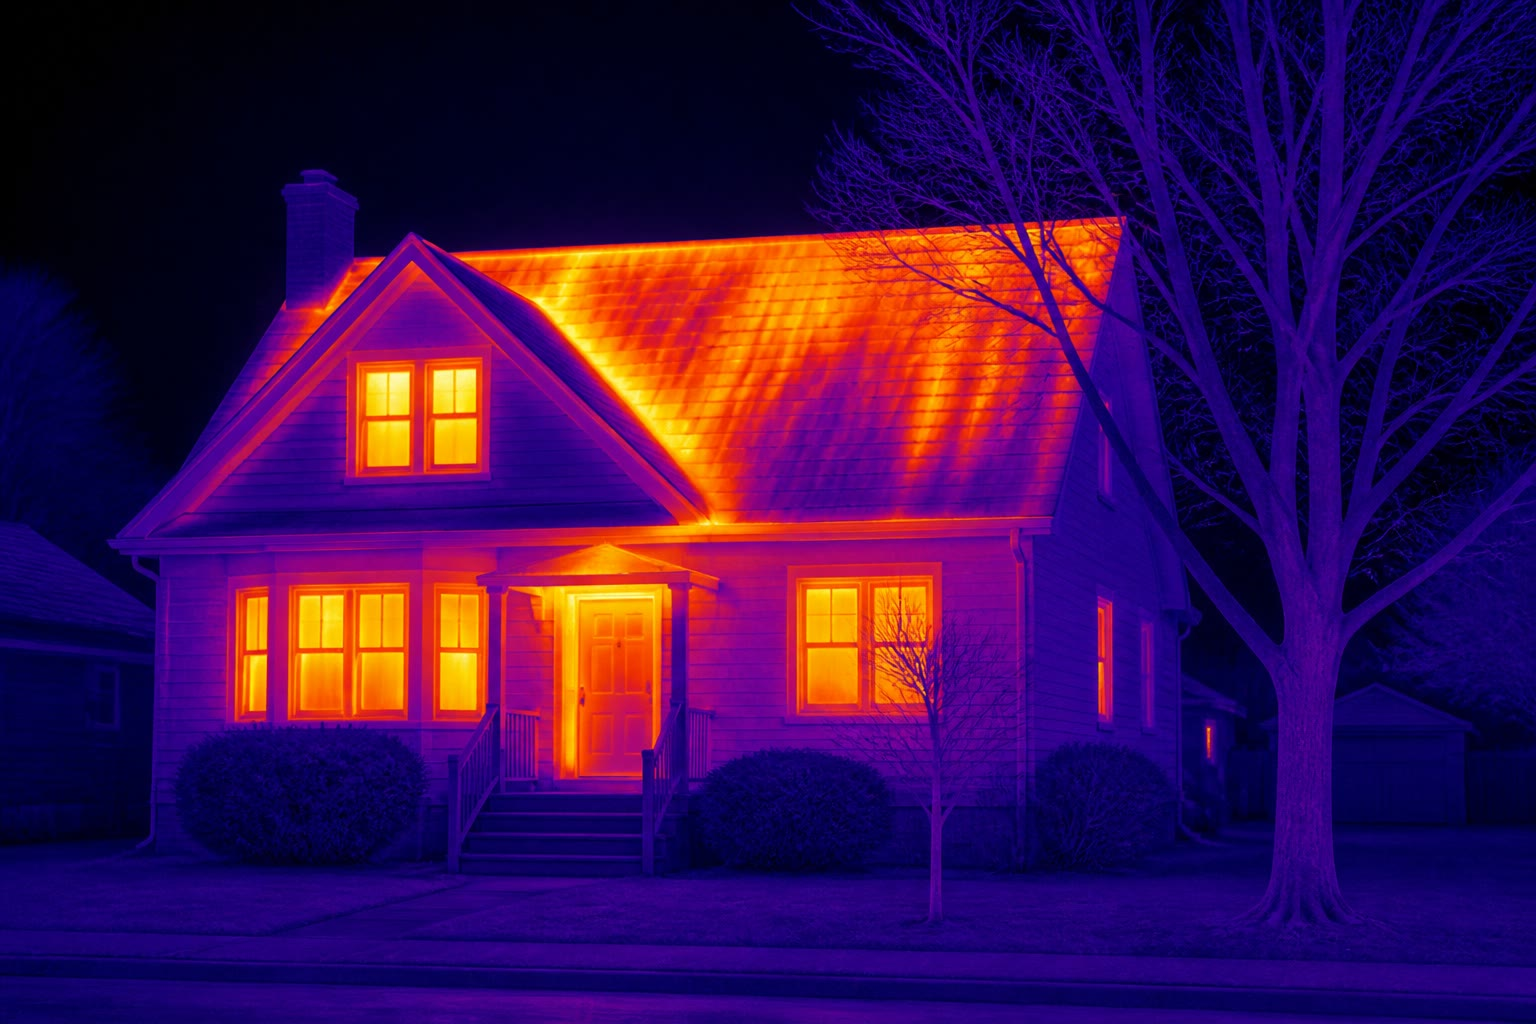
\includegraphics[width=0.58\linewidth]{images/book5/ai/b5-09-thermal-house.jpg}

{\small किसी तापीय कैमरे से देखा गया एक घर: हर सतह अपना प्लांक वर्णक्रम विकिरित करती है, और कैमरा ताप सीधे अवरक्त से पढ़ लेता है --- श्टेफ़ान, बोल्ट्ज़मान और वीन, हीटिंग का बिल जाँचते हुए।}
\end{omfigure}

\section{अभ्यास}

\begin{exercise}[$\star$]\label{exo:b3:photons-phonons:1}
(क) तरंगदैर्घ्य-रूप में प्लांक के नियम से दिखाइए कि शिखर
$\lambda_{\max}T = $ नियतांक मानता है (अतिचरघातांकी समीकरण उद्धृत
किया जा सकता है: $x = 4.965$)। (ख) सूर्य, किसी \qty{2700}{K}
तंतु, किसी \qty{310}{K} पिंड और \qty{2.725}{K} के आकाश के लिए
शिखर-तरंगदैर्घ्य निकालिए। (ग) इन चारों में से किसका नमूना मानव
आँख ठीक से लेती है, और किसी तंतु के उत्पादन का कितना अंश दृश्य
होता है (आकलन: थोड़ा)? (घ) लोगों और इमारतों के लिए ``अवरक्त
कैमरे'' ही सही औज़ार क्यों हैं?
\end{exercise}

\begin{exercise}[$\star$]\label{exo:b3:photons-phonons:2}
विकिरण के बजट। (क) \qty{293}{K} के किसी कमरे में कोई व्यक्ति
($\qty{1.7}{m^2}$, त्वचा
\qty{306}{K}): शुद्ध विकिरित शक्ति
$\sigma A(T_1^4 - T_2^4)$। (ख) उसकी तुलना शरीर के
\qty{100}{W} उपापचय से कीजिए: हम उसे सह क्यों लेते हैं (कपड़े, और
कमरे का वापस विकिरित करना)? (ग) पृथ्वी सूर्य-प्रकाश $\pi
R^2$ पर सोखती है और $4\pi R^2$ पर विकिरित करती है: $T_{\text{प्र}}
= [(1-A)\,\Phi_\odot/4\sigma]^{1/4}$ व्युत्पन्न कीजिए, जहाँ $\Phi_\odot =
\qty{1361}{W/m^2}$ और परावर्तकता $A = 0.30$, और उसका मान निकालिए। (घ)
मापा गया सतही औसत \qty{288}{K} है: उन \qty{33}{K} के अंतर की
क्रियाविधि का नाम लीजिए
(\cref{pb:b3:harmonic-oscillator:1})।
\end{exercise}

\begin{exercise}[$\star$]\label{exo:b3:photons-phonons:3}
फ़ोटॉन गिनना। (क) प्रति घन मीटर $n_\gamma = \num{2.03e7}\,T^3$ के
साथ: \qty{2.725}{K} पृष्ठभूमि का फ़ोटॉन घनत्व।
(ख) पृथ्वी पर सूर्य-प्रकाश: $\Phi_\odot$ और माध्य फ़ोटॉन ऊर्जा
$\approx 2.7\,k_{\text{B}}T_\odot \approx \qty{1.35}{eV}$ से
प्रति वर्ग मीटर प्रति सेकंड फ़ोटॉन-अभिवाह निकालिए। (ग) किसी
\qty{60}{W} तापदीप्त बल्ब (5\% दृश्य) के लिए: प्रति सेकंड दृश्य
फ़ोटॉन। (घ) खगोलविदों के लिए ``फ़ोटॉन गिनना'' रोज़ का काम क्यों है,
पर हीटरों के लिए बेतुका?
\end{exercise}

\begin{exercise}[$\star$]\label{exo:b3:photons-phonons:4}
विपदा और उसकी पूँछ। (क) दिखाइए कि चिरसम्मत ऊर्जा-समविभाजन
(प्रति मोड $k_{\text{B}}T$) $u(\nu) =
8\pi\nu^2k_{\text{B}}T/c^3$ देता है, जो समाकलित करने पर अपसरित हो
जाता है। (ख) \omterm{thm:b3:photons-phonons:planck}{प्लांक का नियम} उस पर कहाँ सिमट आता है? (ग)
रेडियो-खगोलविद CMB को \qty{1.4}{GHz} पर नापते हैं: वहाँ
$h\nu/k_{\text{B}}T \ll 1$ जाँचिए और उनकी ``ऐंटेना ताप'' वाली उस
आदत को उचित ठहराइए, जिसमें तीव्रताएँ केल्विन में बताई जाती हैं। (घ)
CMB के \qty{160}{GHz} शिखर पर
$h\nu/k_{\text{B}}T$ का मान निकालिए: क्या वह शिखर चिरसम्मत है?
\end{exercise}

\begin{exercise}[$\star\star$]\label{exo:b3:photons-phonons:5}
विकिरण दाब। (क) समदैशिकता से $P = u/3$ व्युत्पन्न कीजिए (या गतिक
गुणक मान लीजिए) और पृथ्वी की कक्षा पर सूर्य-प्रकाश का दाब निकालिए;
वायुमंडलीय दाब से तुलिए। (ख) सूर्य के भीतर
($T \approx \qty{1.5e7}{K}$): $P_{\text{rad}} =
aT^4/3$ निकालिए और गैस के दाब $\sim\qty{2e16}{Pa}$ से तुलिए।
(ग) विकिरण दाब $T^4$ की तरह बढ़ता है और गैस का दाब $T$ की तरह:
दिखाइए कि पर्याप्त भारी (और इस तरह अधिक गरम) तारे
विकिरण-प्रधान और अस्थायी क्यों हो जाते हैं --- अर्थात्
$\sim100\,M_\odot$ के पास एडिंगटन की छत। (घ) लेज़र: धकेलने के लिए
केंद्रित कोई \qty{1}{kW} पुंज --- कितना बल? ``कर्षण-किरणें'' फ़िल्मों
में ही क्यों रह जाती हैं, जबकि प्रकाशिक \emph{चिमटियाँ} (प्रवणताएँ,
पिकोन्यूटन) असली औज़ार हैं?
\end{exercise}

\begin{exercise}[$\star\star$]\label{exo:b3:photons-phonons:6}
ब्रह्मांड का खिंचाव। CMB पुनर्योजन पर उत्सर्जित हुई
($T \approx \qty{3000}{K}$, \cref{exo:b3:grand-canonical:12} का
इलाका) और \qty{2.725}{K} पर पहुँचती है। (क) $T \propto
1/a$ से, उत्सर्जन के बाद से सारी लंबाइयों का खिंचाव-गुणक। (ख)
दिखाइए कि हर तरंगदैर्घ्य के एकसमान खिंचाव पर कोई प्लांक वर्णक्रम
प्लांक ही बना रहता है ($T$ का क्या होता है?)। (ग) उत्सर्जित शिखर
(दृश्य नारंगी प्रकाश!) कहाँ आ पहुँचता है? (घ) अतः आकाश आँख को
अँधेरा और किसी सूक्ष्मतरंग ग्राही को दहकता हुआ क्यों दिखता है?
\end{exercise}

\begin{exercise}[$\star\star$]\label{exo:b3:photons-phonons:7}
ध्वनि से डिबाई ताप। (क) ताँबे के लिए $\theta_{\text{D}} =
\hbar c_{\text{s}}(6\pi^2n)^{1/3}/k_{\text{B}}$ का मान निकालिए
($c_{\text{s}} \approx \qty{3800}{m/s}$, $n =
\qty{8.5e28}{m^{-3}}$) और कैलोरीमितीय
\qty{343}{K} से तुलिए। (ख) हीरा: $c_{\text{s}} \approx
\qty{13000}{m/s}$, $n = \qty{1.76e29}{m^{-3}}$: निकालिए और
$\approx\qty{2200}{K}$ से तुलिए। (ग) सीसा: नरम और भारी ---
उसका $\theta_{\text{D}} \approx \qty{90}{K}$ एक वाक्य में
समझाइए। (घ) किसी ठोस की कड़ाई, परमाणविक द्रव्यमान और उसके
क्वांटम-जमाव ताप को जोड़ने वाला नियम बताइए।
\end{exercise}

\begin{exercise}[$\star\star$]\label{exo:b3:photons-phonons:8}
एक केल्विन पर ताँबा। (क) $C = \gamma T + \beta T^3$ का उपयोग
कीजिए, जहाँ $\gamma$ \cref{ex:b3:quantum-statistics:heat} से हो और
डिबाई $T^3$ गुणांक $\theta_{\text{D}} = \qty{343}{K}$ के लिए:
\qty{1}{K} पर प्रति मोल दोनों पद निकालिए। (ख) कौन जीतता है, और
कितने से? (ग) वे किस ताप पर एक-दूसरे को काटते हैं? (घ) यह प्रांत
कैलोरीमितिज्ञ के लिए इलेक्ट्रॉनी \omterm{prop:b3:schrodinger-three-dimensions:counting}{अवस्था घनत्व} की खिड़की
क्यों है?
\end{exercise}

\begin{exercise}[$\star\star$]\label{exo:b3:photons-phonons:9}
एक-परत वाला हरितगृह। मान लीजिए सतह (ताप $T_s$) किसी एक पतली
वायुमंडलीय परत (ताप $T_a$) के नीचे बैठी है, जो सूर्य-प्रकाश के लिए
पारदर्शी है पर तापीय अवरक्त के लिए अपारदर्शी। (क) उस परत के लिए
ऊर्जा-संतुलन लिखिए (वह $\sigma T_s^4$ सोखती और
$2\sigma T_a^4$ विकिरित करती है) और सतह के लिए भी (वह सूर्य-प्रकाश
$S$ तथा $\sigma T_a^4$ सोखती है)। (ख) दिखाइए कि $T_s = 2^{1/4}\,T_{\text{प्र}}$,
जहाँ $\sigma T_{\text{प्र}}^4 = S$। (ग) $T_{\text{प्र}} =
\qty{255}{K}$ के साथ: $T_s$ का मान निकालिए और \qty{288}{K} से
तुलिए (असली वायुमंडल एक आंशिक, बहु-परत वाला कंबल है)। (घ)
\cref{pb:b3:harmonic-oscillator:1} से जोड़िए: कौन-सी आणविक भौतिकी
उस परत को अवरक्त में अपारदर्शी और दृश्य में पारदर्शी बनाती है?
\end{exercise}

\begin{exercise}[$\star\star\star$]\label{exo:b3:photons-phonons:10}
श्टेफ़ान का नियतांक, शुरू से। (क) $u_{\text{कु}} =
\int u(\nu)\dd\nu$ को $x = h\nu/k_{\text{B}}T$ और दिए गए
$\pi^4/15$ के साथ जोड़िए, जिससे $u = aT^4$ मिले, जहाँ $a =
8\pi^5k_{\text{B}}^4/15h^3c^3$। (ख) किसी काली
सतह से अभिवाह $c\,u/4$ होता है (ज्यामितीय चौथाई मान लीजिए):
$\sigma$ बनाइए और उसका मान $h$, $c$,
$k_{\text{B}}$ से संख्यात्मक रूप से निकालिए। (ग) \qty{5.67e-8}{W.m^{-2}.K^{-4}} से तुलिए।
(घ) ऐतिहासिक उलटाव: प्लांक ने अपना नियम वर्णक्रमों पर बैठाया और
$h$ तथा $k_{\text{B}}$ \emph{दोनों} निकाल लिए (और इस तरह अवोगाद्रो
की संख्या भी), 1900 में --- बताइए कि कृष्णिका वक्र एक साथ दो
नियतांक क्यों बाँध देता है।
\end{exercise}

\begin{exercise}[$\star\star\star$]\label{exo:b3:photons-phonons:11}
आइंस्टाइन के A और B (1917)। द्वि-स्तरीय परमाणु (ऊर्जाएँ $0,
h\nu_0$; जनसंख्याएँ $N_1, N_2$) वर्णक्रमीय घनत्व
$u(\nu_0)$ वाले विकिरण में बैठे हैं। अवशोषण दर: $B_{12}uN_1$;
उद्दीपित उत्सर्जन: $B_{21}uN_2$; स्वतःस्फूर्त: $AN_2$। (क) संतुलन
का समीकरण लिखिए। (ख) माँगिए कि बोल्ट्ज़मान अनुपात
$N_2/N_1 = \eu^{-h\nu_0/k_{\text{B}}T}$ और प्लांक का $u$
\emph{सभी} $T$ के लिए एक साथ टिकें: इससे $B_{12} = B_{21}$
व्युत्पन्न कीजिए, और
\[
\frac{A}{B} = \frac{8\pi h\nu_0^3}{c^3} .
\]
(ग) व्याख्या कीजिए: तापीय संतुलन स्वतःस्फूर्त उत्सर्जन का होना
\emph{क्यों} अनिवार्य कर देता है, और उसकी दर उद्दीपित वाली से
क्यों तय कर देता है? (घ) वह $\nu^3$:
\cref{exo:b3:perturbation-theory:8} के जीवनकालों से जोड़िए, और यह
भी कि एक्स-किरण आवृत्तियों पर लेज़िंग कठिन क्यों है।
\end{exercise}

\begin{exercise}[$\star\star\star$]\label{exo:b3:photons-phonons:12}
हीरा, फ़ोनॉनों का राजमार्ग। किसी विद्युत्रोधी की ऊष्मा चालकता:
प्रति आयतन $\kappa = \tfrac13 C_v c_{\text{s}}\ell$, जहाँ
$\ell$ फ़ोनॉन का माध्य मुक्त पथ है। (क) \qty{300}{K} पर हीरे के
लिए ($C_v \approx \qty{1.8e6}{J.m^{-3}K^{-1}}$, अर्थात्
आंशिक रूप से जमा हुआ; $c_{\text{s}} = \qty{13000}{m/s}$; $\ell
\approx \qty{0.3}{\micro m}$): $\kappa$ निकालिए और ताँबे के
\qty{400}{W/(m.K)} से तुलिए। (ख) हीरे में $\ell$ इतना लंबा क्यों है
(कड़ा, हलका, समस्थानिक रूप से स्वच्छ --- फ़ोनॉनों को प्रकीर्ण कौन
करता है?)। (ग) समस्थानिक रूप से शुद्ध किया गया हीरा $\kappa$ को
लगभग दुगना कर देता है: यह समस्थानिक द्रव्यमान-अव्यवस्था से होते
फ़ोनॉन-प्रकीर्णन के बारे में क्या बताता है? (घ) दो उपयोग:
इलेक्ट्रॉनिकी में ऊष्मा फैलाने वाली परतें; और कोई हीरा होंठ को
ठंडा क्यों लगता है --- उस अनुभूति को समझाइए।
\end{exercise}

\begin{omfigure}
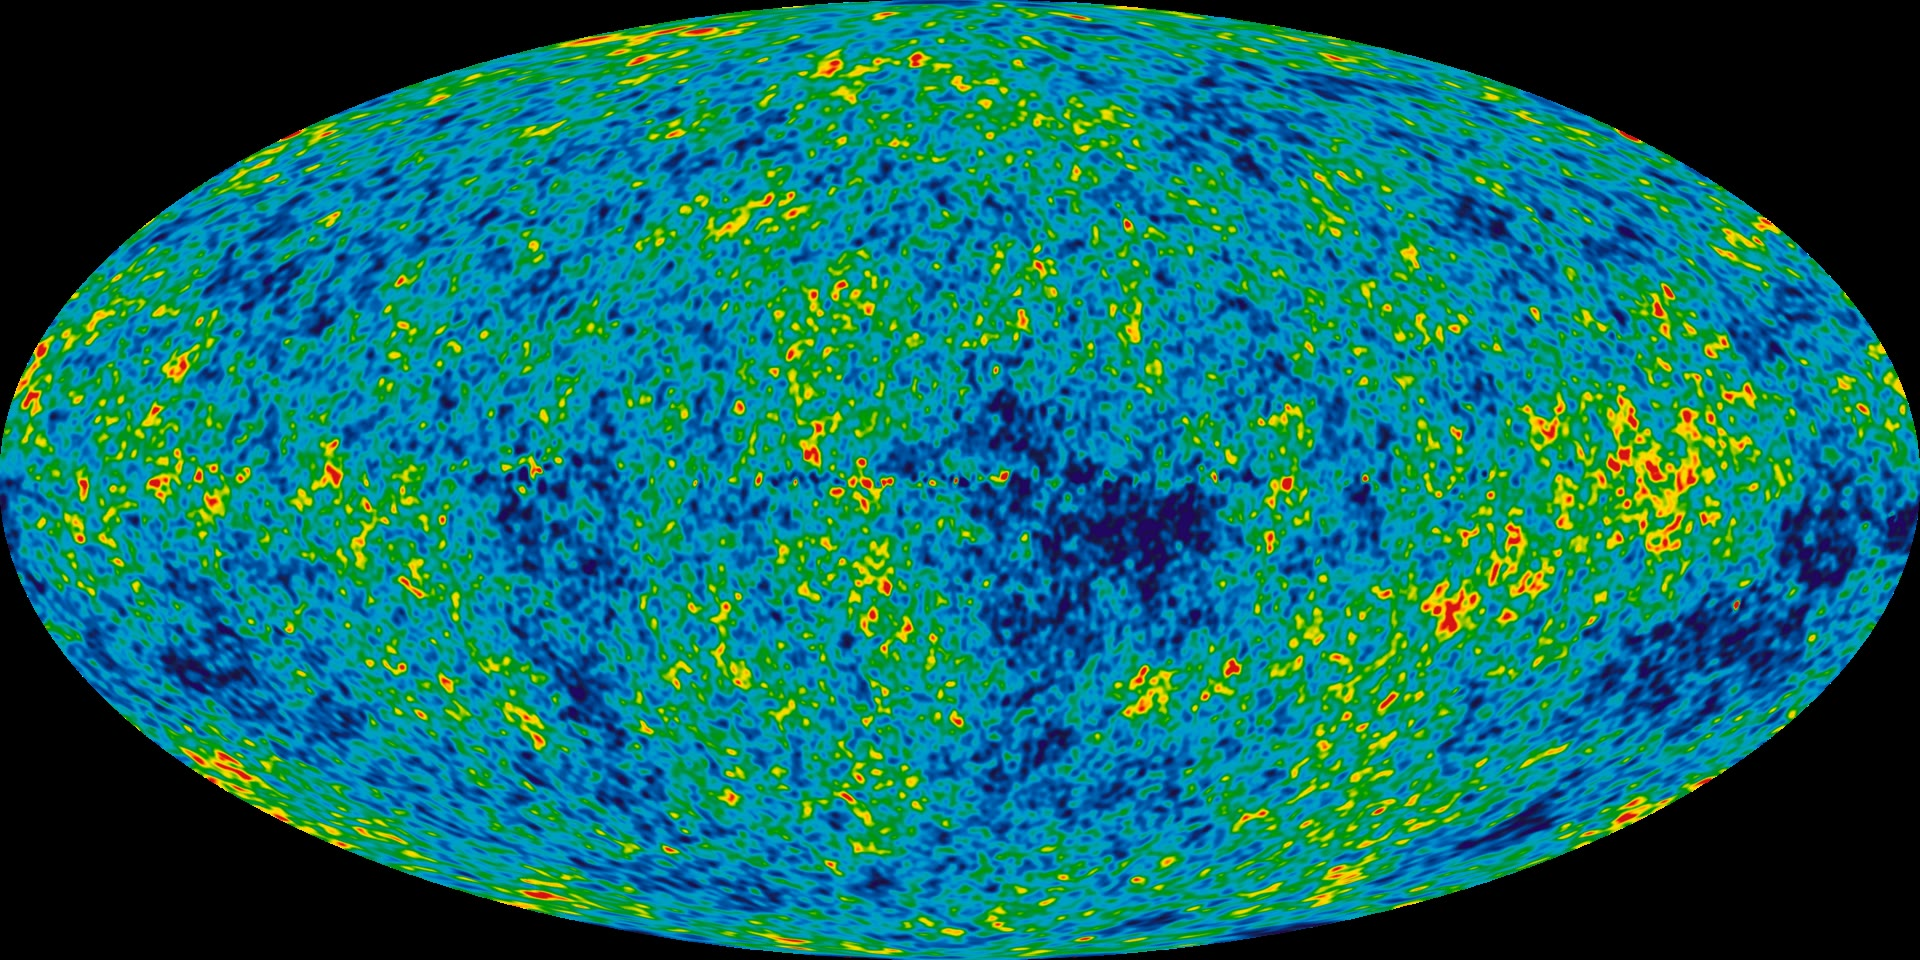
\includegraphics[width=0.62\linewidth]{images/book5/photo-cmb-wmap.jpg}

{\small सूक्ष्मतरंगों में पूरा आकाश (NASA/WMAP, सार्वजनिक डोमेन): ब्रह्मांडीय पृष्ठभूमि का \qty{2.7}{K} प्लांक विकिरण, मानचित्रित। वह चितकबरापन एक भाग प्रति $10^5$ का है --- आकाशगंगाओं के बीज, इस अध्याय की कृष्णिका पर छपे हुए।}
\end{omfigure}

\section{समस्या: सबसे पुराना प्रकाश}

\begin{problem}[{सप्ताहांत समस्या --- ब्रह्मांडीय सूक्ष्मतरंग
पृष्ठभूमि पढ़ना}]\label{pb:b3:photons-phonons:1}
किसी भी मिलीमीटर-तरंग ग्राही को आकाश के किसी भी टुकड़े की ओर
मोड़िए, वह वही संकेत बताता है: $T =
\qty{2.72548(57)}{K}$ पर एक प्लांक वर्णक्रम, जो मनुष्य की बनाई किसी
भी भट्ठी से चिकना है। यह ब्रह्मांड के पुनर्योजन
(\cref{exo:b3:grand-canonical:12}) की कौंध है, जो ग्यारह सौ गुना
खिंच चुकी है, और वह ब्रह्मांड की जनगणना ढोती है। आँकड़े: $T_0 =
\qty{2.725}{K}$; $n_\gamma = \num{2.03e7}\,T^3\,\unit{m^{-3}}$;
$u = aT^4$, $a = \qty{7.56e-16}{J.m^{-3}.K^{-4}}$; आज का बैरिऑन
घनत्व $n_{\text{b}} \approx \qty{0.25}{m^{-3}}$; क्रांतिक घनत्व
$\rho_{\text{c}} \approx \qty{8.6e-27}{kg/m^3}$।

\medskip\noindent\textbf{भाग I --- वर्णक्रम।}
\begin{enumerate}
  \item CMB का शिखर (वीन) तरंगदैर्घ्य और प्रति घन सेंटीमीटर उसका
        फ़ोटॉन घनत्व निकालिए।
  \item उसका ऊर्जा घनत्व $\unit{J/m^3}$ में और
        $\unit{eV/cm^3}$ में निकालिए, तथा क्रांतिक घनत्व में उसका
        द्रव्यमान-तुल्य अंश भी।
  \item COBE का वर्णक्रम (1990) प्लांक से
        $10^4$ में कुछ भागों तक मिला --- दर्शकों ने उस आलेख पर
        तालियाँ बजाईं। खाली आकाश से आते किसी \emph{पूर्णतः तापीय}
        वर्णक्रम को किसी तप्त सघन अतीत के सिवा और कुछ मानकर समझाना
        इतना कठिन क्यों है?
  \item उत्सर्जन के समय वही फ़ोटॉन \qty{3000}{K} की कृष्णिका बनाते
        थे: खिंचाव-गुणक $1 + z =
        T_{\text{तब}}/T_0$ जाँचिए।
  \item ब्रह्मांड ठीक उसी ताप पर पारदर्शी क्यों हो गया
        (\cref{ch:b3:grand-canonical} का कौन-सा संतुलन बंद हो गया,
        यह याद कीजिए)?
  \item रात का आकाश अँधेरा है (पुराने खगोल का ओल्बर्स विरोधाभास):
        वह ठीक किस अर्थ में वस्तुतः \emph{चमकीला} है --- किस
        तरंगदैर्घ्य और किस ताप पर?
\end{enumerate}

\medskip\noindent\textbf{भाग II --- जनगणना।}
\begin{enumerate}[resume]
  \item फ़ोटॉन-से-बैरिऑन अनुपात $\eta^{-1} =
        n_\gamma/n_{\text{b}}$ निकालिए।
  \item वह संख्या --- प्रति प्रोटॉन लगभग दो अरब फ़ोटॉन ---
        ब्रह्मांड-विज्ञान के मूल आँकड़ों में से एक है: बताइए कि वह
        पदार्थ--प्रतिपदार्थ असममिति के बारे में क्या नापती है
        (\cref{exo:b3:grand-canonical:12} याद कीजिए: फ़ोटॉन
        अधिकतर विनाश के उत्पाद हैं)।
  \item CMB के ऊर्जा घनत्व की तुलना तारा-प्रकाश के घनत्व
        ($\sim\qty{2e-15}{J/m^3}$, पूरे ब्रह्मांड पर औसत) से कीजिए:
        ब्रह्मांड में कौन-सा प्रकाश हावी है?
  \item फ़ोटॉनों में CMB उन सबसे भारी है जो तारे कभी चमके हैं:
        इससे आरंभिक ब्रह्मांड ``विकिरण-प्रधान'' क्यों हो जाता है,
        और बाद में किसने कमान सँभाली ($T^4$ बनाम $T^3$ के मापन,
        पदार्थ के $a^{-3}$ के सामने)?
  \item पदार्थ--विकिरण समता के युग का आकलन कीजिए: विकिरण-घनत्व
        $(1+z)^4$ की तरह और पदार्थ $(1+z)^3$ की तरह मापित होते
        हुए, और आज का अनुपात
        $u_{\text{rad}}/\rho_{\text{m}}c^2 \approx 1/3400$ लेकर,
        $z_{\text{सम}}$ खोजिए।
  \item न्यूट्रिनो पहले वियुग्मित हुए और ज़रा अधिक ठंडे हुए
        (वे \cref{exo:b3:grand-canonical:12} वाले $e^+e^-$ विनाश
        के पुनर्तापन से चूक गए): पूर्वकथित
        $T_\nu = (4/11)^{1/3}T_\gamma$ --- उसका मान निकालिए, और
        \qty{1.95}{K} के उस न्यूट्रिनो सागर की भविष्यवाणी पर चकित
        होइए, जिसे अब तक किसी ने सीधे नहीं पकड़ा।
\end{enumerate}

\medskip\noindent\textbf{भाग III --- विषमदैशिकताएँ।}
\begin{enumerate}[resume]
  \item CMB एक दिशा में \qty{3.4}{mK} अधिक गरम और उलटी दिशा में
        ठंडी है: \cref{ch:b3:relativistic-kinematics} की डॉप्लर
        भौतिकी से इसकी व्याख्या कीजिए और हमारा
        वेग निकालिए ($\Delta T/T = v/c$)।
  \item वह द्विध्रुव हटा देने पर $\Delta T/T \sim
        \num{e-5}$ की लहरें बच रहती हैं (COBE 1992, फिर WMAP,
        प्लांक): वे $z = 1100$ पर किसका मानचित्र बनाती हैं?
  \item वे $10^{-5}$ घनत्व-बीज बढ़कर आकाशगंगाएँ बने: गुरुत्व
        अधिघनत्वों को क्यों बढ़ाता है (कौन-सी अस्थिरता), और उस
        वृद्धि को सचमुच शुरू होने के लिए पदार्थ--विकिरण समता की
        ज़रूरत क्यों पड़ी?
  \item सबसे प्रबल लहर का आकार (आकाश पर लगभग एक अंश) एक ध्वनिक
        तरंगदैर्घ्य है --- फ़ोटॉन--बैरिऑन प्लाज़्मा में ध्वनि (इस
        अध्याय की गैस और
        \cref{ch:b3:continuum-elasticity} की तरंगें, दोनों!): उसका
        पैमाना क्या तय करता है (पुनर्योजन से पहले ध्वनि कितनी दूर
        जाती है)?
  \item उस कोण को ज्ञात भौतिक पैमाने के सामने नापना ब्रह्मांड की
        ज्यामिति त्रिकोणित कर देता है: परिणाम बताइए (समतल, प्रतिशत
        की परिशुद्धि तक)।
  \item \qty{2.7}{K} का एकध्रुव, \qty{3}{mK} का द्विध्रुव,
        \num{e-5} की लहरें: हर एक ने क्या सिखाया, क्रम में रखिए
        (एक तप्त अतीत; हमारी गति; और हर चीज़ के बीज तथा ज्यामिति)।
\end{enumerate}

\medskip\noindent\textbf{भाग IV --- विरासत।}
\begin{enumerate}[resume]
  \item पेंज़ियास और विल्सन को यह संकेत 1965 में न हटने वाले
        ऐंटेना-शोर के रूप में मिला (कबूतरों को भगाने के बाद):
        \qty{3}{K} पर कोई \emph{समदैशिक}, ऋतु-निरपेक्ष आधिक्य किसी
        भी स्थानीय या आकाशगंगीय स्रोत से अव्याख्येय क्यों था?
  \item किसी बेसुरे अनुरूप टेलीविज़न के स्थैतिक शोर का लगभग $1\%$
        यही संकेत था: एक वाक्य में विचार कीजिए।
  \item CMB आकाशगंगा-गुच्छों से होकर गुज़रती है और तप्त
        इलेक्ट्रॉन उसे ज़रा ऊँची आवृत्ति की ओर धकेल देते हैं
        (सुन्याएव--ज़ेल्दोविच प्रभाव): इससे गुच्छ कम आवृत्ति पर
        \emph{छायाओं} के रूप में क्यों दिखते हैं, और ऐसी छाया का
        विशेष गुण क्या है (दूरी से स्वतंत्र)?
  \item आज की अग्रिम पंक्ति CMB के ध्रुवण में आदिम गुरुत्व-तरंगों
        की छाप खोज रही है: वह खोज इस पुस्तक के कौन-से अध्यायों का
        विवाह करा देती
        (\cref{ch:b3:covariant-electromagnetism} का ध्रुवण,
        गुरुत्व की तरंगें)?
  \item अपने शरीर से होकर गुज़रते CMB फ़ोटॉनों का अभिवाह निकालिए
        (प्रति एकांक क्षेत्रफल $n_\gamma c/4$, शरीर का \omterm{def:b3:scattering-theory:cross-section}{अनुप्रस्थ काट}
        $\sim\qty{0.5}{m^2}$): महाविस्फोट के कितने अवशेष
        प्रति सेकंड आपको पार करते हैं?
  \item CMB एक विराम-तंत्र चुन लेती है (वही, जिसमें द्विध्रुव
        लुप्त हो जाता है): समझाइए कि यह आपेक्षिकता का खंडन क्यों
        \emph{नहीं} करता --- यह कैसा तंत्र है, जिसे नियम नहीं बल्कि
        पदार्थ-सामग्री वरीयता देती है?
  \item नामित परिणाम का सार दीजिए: आकाश को भरता $2.725$ केल्विन
        का प्लांक वक्र --- प्रति घन सेंटीमीटर $411$ फ़ोटॉन, प्रति
        बैरिऑन दो अरब, शिखर \qty{160}{GHz} पर --- उस तप्त आरंभ की
        तापीय रसीद है: सांख्यिकीय भौतिकी, ब्रह्मांड-विज्ञान की
        आधारशिला के रूप में।
\end{enumerate}
\end{problem}
